\section{Imaging}


\subsection{Image Reconstruction}

The inverse Fourier transform of the complex visibilities in the $(u,v)$ plane (Equation \ref{eq: V(u,v)}), given by the equation:
\begin{equation}
    I(l,m) = \int_{-\infty}^\infty V(u,v) e^{2\pi i(ul+vm)}dudv,
    \label{eq: I(l, m)}
\end{equation}
\noindent converts the visibilities into the image domain \citep{Thompson}. Since the \uv coverage is incomplete, this produces a `dirty image', rather than a perfect reconstruction. The dirty image is the true sky brightness distribution convolved with the point spread function of the interferometer, called the `dirty beam' \citep{Marvil2026}.


%%%%%%%%%%%%%%%%%%%%%%%%%%%%%%%%%%%%%%%%%%%%%%%%%%%
%%%%%%%%%%%%%%%%%%%%%%%%%%%%%%%%%%%%%%%%%%%%%%%%%%%


\subsection{Deconvolution (\texttt{clean}) and Weighting Schemes}
\label{sec: inter_weighting}
% ------------------------------------------------


Deconvolution is the process of reducing the effects of the dirty beam in the dirty image, typically using the algorithm \clean \citep{Thompson, Marvil2026}. The \clean algorithm iteratively builds a model of the image from delta functions or small Gaussian components. At each iteration, the brightest point of the dirty image is located, a scaled copy of the dirty beam centred on this point is subtracted, and the position and brightness are recorded as \clean components \citep{Monnier}. This process is repeated iteratively until only the residual noise is left. The \clean model is then convolved with the final \clean beam, called the synthesized beam, which is a smooth Gaussian with the same full width at half maximum (FWHM) as the dirty beam. The residual image is added to the restored image, producing the final \clean image \citep{Thompson}. An example of a dirty versus clean image can be seen in Figure \ref{fig: Dirty_vs_clean}. 


\begin{figure}[htbp]
  \centering
  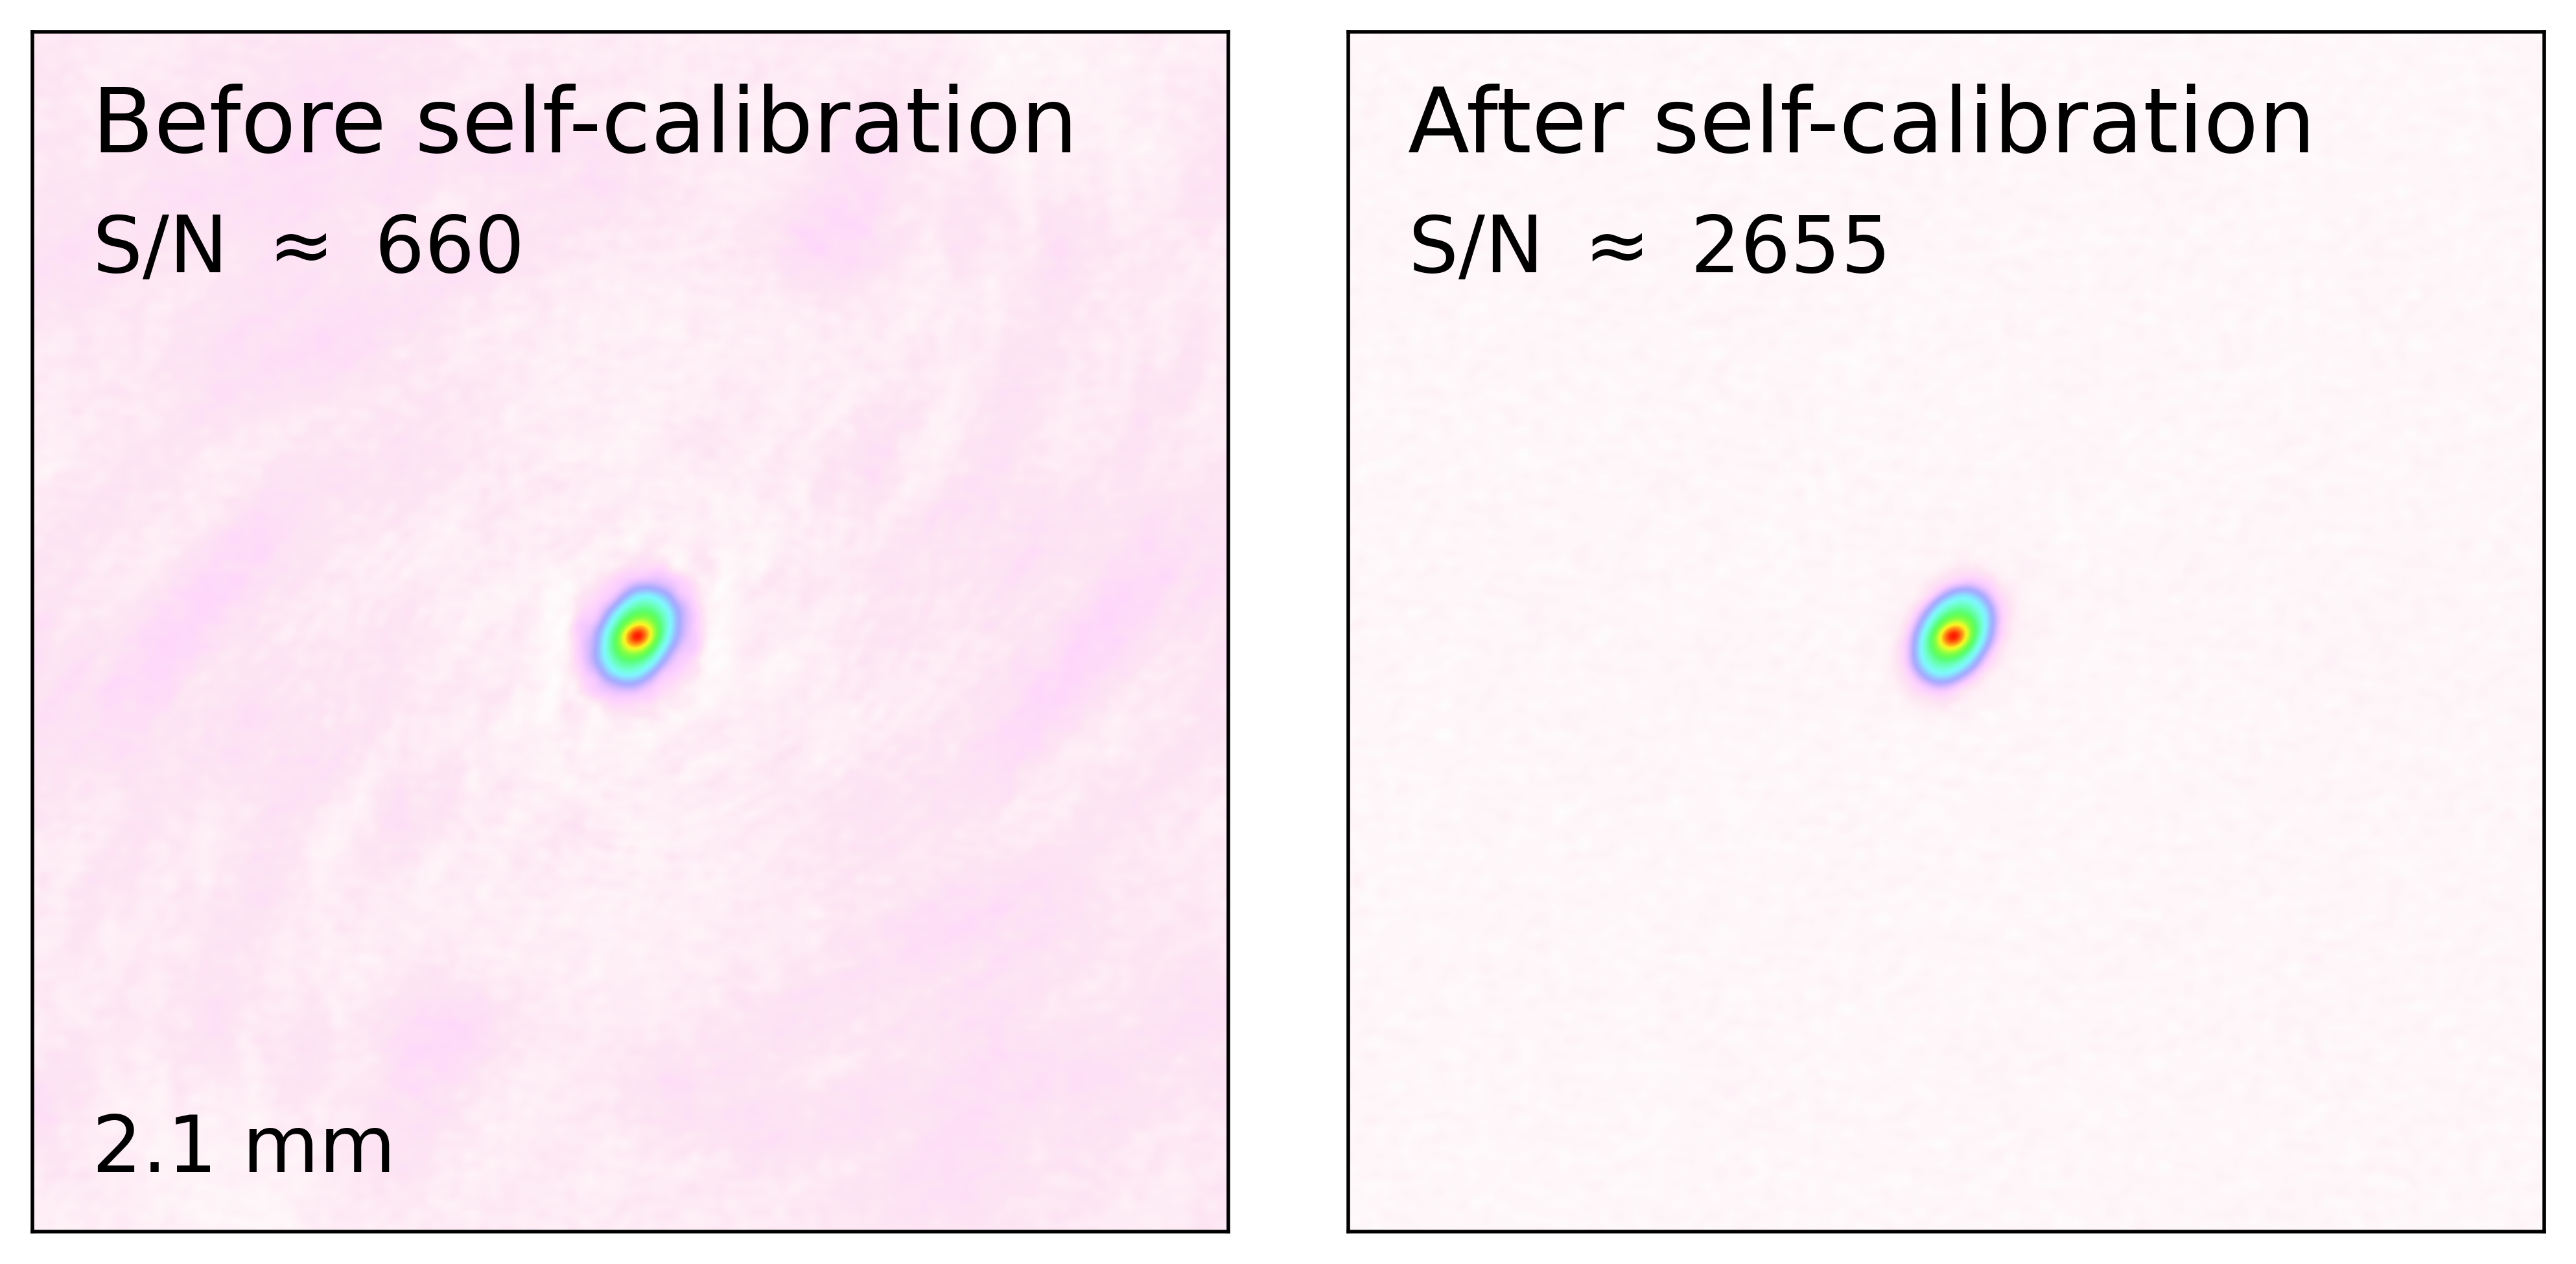
\includegraphics[width=0.99\textwidth]{WRITEUP_AND_IMAGES/IMAGES/WRITEUP/BeforeAndAfterClean.png}
  \caption[\note{add short caption after plot is finalized}]{\note{THIS IS NOT THE REAL IMAGE! Just a placeholder for formatting purposes.}\question{Do I have access to a pre-clean image of IRS 63 or is this something I will need to get from a different source? (I will add a caption too).}}
  \label{fig: Dirty_vs_clean}
\end{figure}




When using the \texttt{clean} algorithm, each visibility in the \uv plane is assigned a weight, which influences the properties of the dirty beam and the resulting image \citep{Marvil2026}. When each visibility is weighted equally, this is called \emph{natural weighting}, which gives the highest sensitivity and therefore best signal-to-noise ratio (\SNRns) for detecting faint objects but with a lower resolution \citep{Monnier, Thompson}. When visibilities are weighted by visibility density in the \uv plane, such that well-sampled regions are given less weight than less-sampled regions, this is called \emph{uniform weighting}. Since the \uv plane is generally more densely sampled at shorter \uv distances, uniform weighting weighs the longer \uv distances higher. This produces a smaller synthesized beam and therefore higher angular resolution, but with lower sensitivity as a trade-off \citep{Monnier}.


A `robust' parameter was introduced in \cite{briggs} for a weighting scheme called Briggs weighting. The robust parameter controls a balance between natural and uniform weighting to find an ideal trade-off between sensitivity and angular resolution \citep{Monnier, Marvil2026}. The robust parameter ranges from -2 to 2, where more negative values have weighting closer to uniform weighting, and more positive values produce weighting closer to natural weighting \citep{Thompson}.

%%%%%%%%%%%%%%%%%%%%%%%%%%%%%%%%%%%%%%%%%%%%%%%%%%%





%%%%%%%%%%%%%%%%%%%%%%%%%%%%%%%%%%%%%%%%%%%%%%%%%%%
\subsection{Self-Calibration}

Self-calibration is an additional calibration step that can be performed after standard calibration. In standard calibration, calibration sources such as quasars are used to determine instrumental and atmospheric effects. In self-calibration, the science target itself is used as the calibrator to further correct both the phase and amplitude of the data. Because of this, the target needs to be bright, with a \SNR $\gtrsim$ 100. 


The signal recieved by each antenna can be affected by time-dependent atmospheric variations, which can introduce additional calibration errors. Self-calibration is useful for reducing artifacts caused by these errors, as well as artifacts from a background source due to direction-independent calibration errors \citep{Marvil2}. The specific details on the self-calibration process used in this project are described in Chapter \ref{ch_data}. 






%%%%%%%%%%%%%%%%%%%%%%%%%%%%%%%%%%%%%%%%%%%%%%%%%%%
% The clean bean is a Gaussian fit to the central peak of the PSF \citep{Marvil2026}. 

% \quoted{The dirty image is the inverse transiform of the measured visibilities, which is typicall created by evaluating the visibilities on a regular grid, then using the Fast Fourier Transform} \citep{Marvil2026}. 




% Primary beam is determined by the size of the dish \citep{Ludovici2026}. 

% The synthesized bean is determined by the separation of the telescope \citep{Ludovici2026}. 


% The dirty bean (PSF) is the result of the system to a point source \citep{Ludovici2026}. 


% The point spread function (PSF) is a convolutional image feature due to incomplete UV sampling (dirty beam) \citep{Marvil2026}. The PSF is \quoted{what every point source looks like in the dirty image (also called the dirty beam), it is the Fourier transofrm of th gridded wrights.} \citep{Marvil2026}. 


% However, before this is done we need to learn about the observation conditions, via the phase stability \citep{Marvil2}. To do this, you identidt a long scan on a nright calibrator (bandpass) and plot the phase vs. time for a single baseline \citep{Marvil2}. What we look for is a coherence time (peak to peak time) to be $\lessim 1$ minuite. 

%%%%%%%%%%%%%%%%%%%%%%%%%%%%%%%%%%%%%%%%%%%%%%%%%%%


